\documentclass[serif ,mathserif, 8pt]{beamer}
\usepackage{pxfonts}
%\usepackage{eulervm}


%%-------------------------
%  ---- BEAMER THEME ---
%%--------------------------
\usetheme{AnnArbor}
\usecolortheme{crane}
\setbeamercovered{transparent}
%\setbeamercolor{section in head/foot}{use=structure,bg=structure.fg!55!bg}
\setbeamerfont{frametitle}{series=\bfseries} % Frame titles should be bold
\useinnertheme[shadow=true]{rounded}
\useoutertheme[subsection=true]{smoothbars}%Beamer Outer Theme-circles on top
%\useinnertheme{circles} %rectangle bullet points instead of circle ones
%\mode<presentation>
%\newcommand*\oldmacro{}%
%\let\oldmacro\insertshorttitle%
%\renewcommand*\insertshorttitle{%
%  \oldmacro\hfill%
%  \insertframenumber\,}%/\,\inserttotalframenumber
%\setbeamertemplate{footline}[frame number]
%%-------------------------------------------------------------------

\usepackage[utf8]{inputenc}
\usepackage[english]{babel}
\usepackage[T1]{fontenc}
\usepackage{amsmath}
\usepackage{graphicx}
\usepackage{url}
\usepackage{xcolor}
\usepackage{hyperref}
\hypersetup{
	colorlinks = true, linkcolor=blue!45!black, citecolor=black, anchorcolor=green,
	pdfstartview=FitH, pdffitwindow=true, pdfmenubar=true,
	pdfcreator=PDFLaTeX, pdfproducer=PDFLaTeX, 
	pageanchor=true, backref,
	hyperindex=true}
\usepackage{multimedia,animate}
%\usepackage{xmpmulti}
\usepackage{media9}
\usepackage{ragged2e}
\usepackage{wasysym}

\author{\textbf{A. Ammar*, H. Ghalila, S. Varadharajan, Y. Majdi, S. Lahmar, Z Dhaoudi, M. Zghal, Zohra Ben Lakhdar, V. Lakshminarayanan*}}
\title{Hands-on experimental and computer laboratory in optics}
\subtitle{The Young Double Slit Experiment}
\setbeamercovered{transparent} 
%\setbeamertemplate{navigation symbols}{} 
%%%%%%%%%%%%%%%%%%%%%%%%%%%%%%%%  L O G O   %%%%%%%%%%%%%%%%%%%%%%%%%%%%%%%
%\logo{%
%    
\includegraphics[width=1cm,height=0.8cm,keepaspectratio]{images/logoLSAMA}%
   % \includegraphics[width=1cm,height=1cm,keepaspectratio]{images/logoH}~%
    %\includegraphics[width=1cm,height=1cm,keepaspectratio]{logo3}%
%}

\institute[LSAMA Lab \& Optical Society of Tunisia]{
\includegraphics[width=3cm]{images/STO_logo} 
\includegraphics[width=1.5cm]{images/logoLSAMA} \\
Optical Society of Tunisia \& LSAMA Lab, Faculty of Sciences of Tunis}
%%%%%%%%%%%%%%%%%%%%%%%%%%%%%%%%%%%%%%%%%%%%%%%%%%%%%%%%%%%%%%%%%%%%
%\institute{} 
\date{\today} 
%\subject{} 
\usepackage[style=verbose-note,autocite=footnote,abbreviate=true]{biblatex}
%\usepackage{filecontents}

\begin{document}
\begin{frame}
\titlepage
\end{frame}
\begin{frame}{Teaching has not changed over the centuries!}
		\centering
		\begin{figure}
			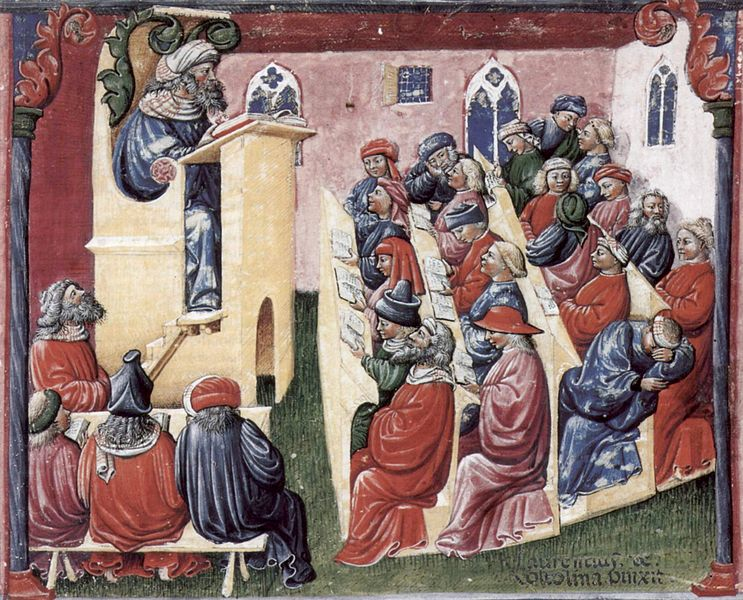
\includegraphics[width=.65\linewidth]{images/Laurentius_de_Voltolina_001}
			\caption{Henry of Germany lecturing at the University of Bologna. Painting by Laurentius de Voltolina (1350).}
		\end{figure}
		
\end{frame}

\begin{frame}{Active learning cycle}
	\begin{columns}[c]
		\begin{column}{0.6\textwidth}
			\begin{block}{What teacher need?}
				Teacher/Learner needs a crucial tool to animate his class:
				\begin{itemize}
					\item Low-cost equipment and techniques that are suitable for physics education in many developing countries.
					\item Easy to build and to use.
				\end{itemize}
				
			\end{block}
				
				
		\begin{exampleblock}<2->{Example: ALOP}
			Active Learning in Optics and Photonics (ALOP) UNESCO’s programme is the best example for this concept that provide a set of experiments to understand optics and photonics.
		\end{exampleblock}
		\begin{alertblock}<3->{Computations}
			ALOP does not contain computations. Nowadays, science is not only the classic two divisions: Theory and Experiment.
		\end{alertblock}
		\end{column}
		\begin{column}{0.4\textwidth}
			\begin{figure}
				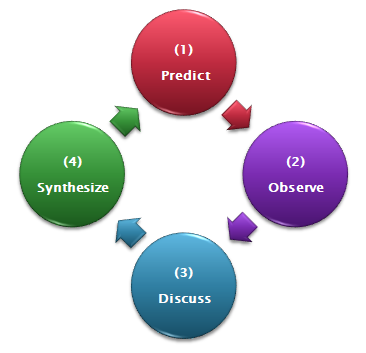
\includegraphics[width=\linewidth]{images/alop_cycle}
				\caption{ALOP learning cycle.}
			\end{figure}
		\end{column}
	\end{columns}
		
\end{frame}

\begin{frame}{Active Learning in Simulating Optics (ALSO)}
\begin{columns}[c]
	\begin{column}{0.6\textwidth}
	\begin{block}{The role of computing in science}
			Scientific computing is often closely related to theory, but it also has many characteristics in common with experimental work.\\
		It is therefore often viewed as a new third branch of science.\\
		
		Nowadays a vast majority of both experimental and theoretical papers involve some numerical calculations, simulations or computer modeling.\\
		To start computing we need to learn a programming language.\\
	\end{block}

	
		
	\end{column}
	\begin{column}{0.4\textwidth}
		\begin{figure}
			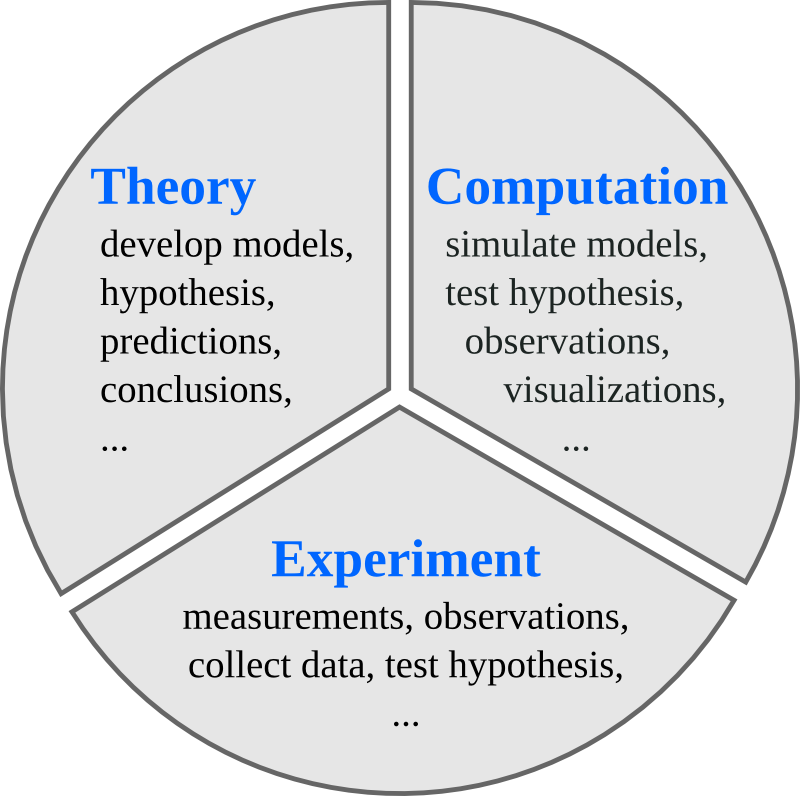
\includegraphics[width=\linewidth]{images/theory-experiment-computation}
			\caption{Three branch of science.}
		\end{figure}
	\end{column}
\end{columns}

\end{frame}

\begin{frame}{Python}
\begin{columns}[c]
	\begin{column}{0.6\textwidth}
		Python is a modern, general-purpose, object oriented, high-level programming language.
		
		General characteristics of Python:
		
		Clean and simple language: Easy-to-read and intuitive code, easy-to-learn minimalistic syntax, maintainability scales well with size of projects.
		
		Expressive language: Fewer lines of code, fewer bugs, easier to maintain.
	\end{column}
	
	\begin{column}{0.4\textwidth}
		\begin{figure}
			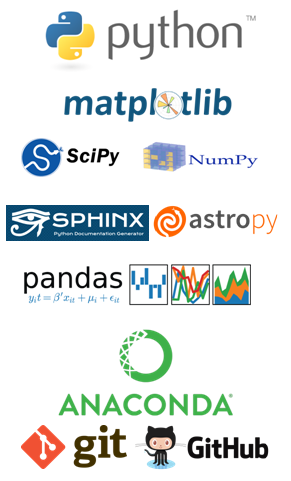
\includegraphics[width=.8\linewidth]{images/python}
		\end{figure}
	\end{column}
\end{columns}

\end{frame}

\begin{frame}{Example: The Young Double Slit Experiment}
	\begin{block}{ALOP, Zimbabwe, July 2018}
		\centering
		\begin{figure}
			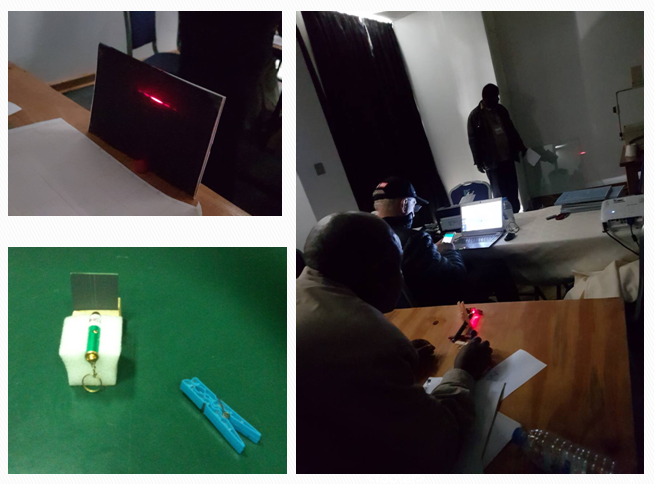
\includegraphics[width=.7\linewidth]{images/alop2018}
		\end{figure}
	\end{block}
\end{frame}
\begin{frame}{Observation}
	\centering
	\begin{figure}
		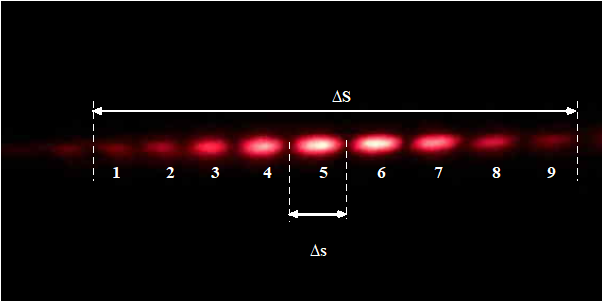
\includegraphics[width=.7\linewidth]{images/Image1}
		\caption{Measures of the size of the main central peak of diffraction $\Delta S$, the size of the small spot du to the interferences $\Delta s$ and enumeration of the number of interference peak inside the main peak of diffraction
		}
	\end{figure}
The distance D acts as an input parameter and except for this parameter, which can be easily varied and measurable, the slit width and the distance between them are made imprecise or even unknown. All these parameters will be used when comparing experiments and numerical modeling and as goal of the experiment is to determine precisely these last two parameters ($\Delta S$ and $\Delta s$). 

\end{frame}
\begin{frame}{Numerical modeling}
\begin{columns}[c]
	\begin{column}{0.6\textwidth}
		\begin{figure}
			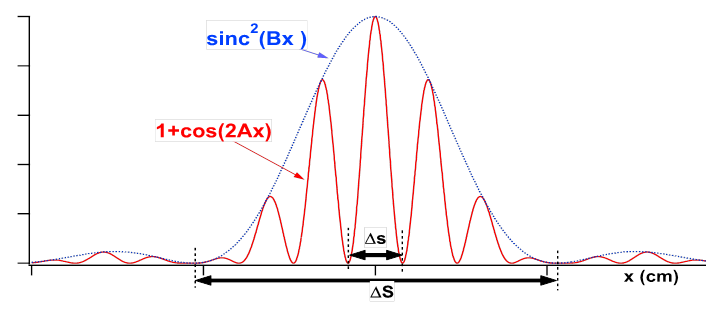
\includegraphics[width=\linewidth]{images/im2}
		\end{figure}
	\end{column}
	
	\begin{column}{0.4\textwidth}
			\begin{figure}
			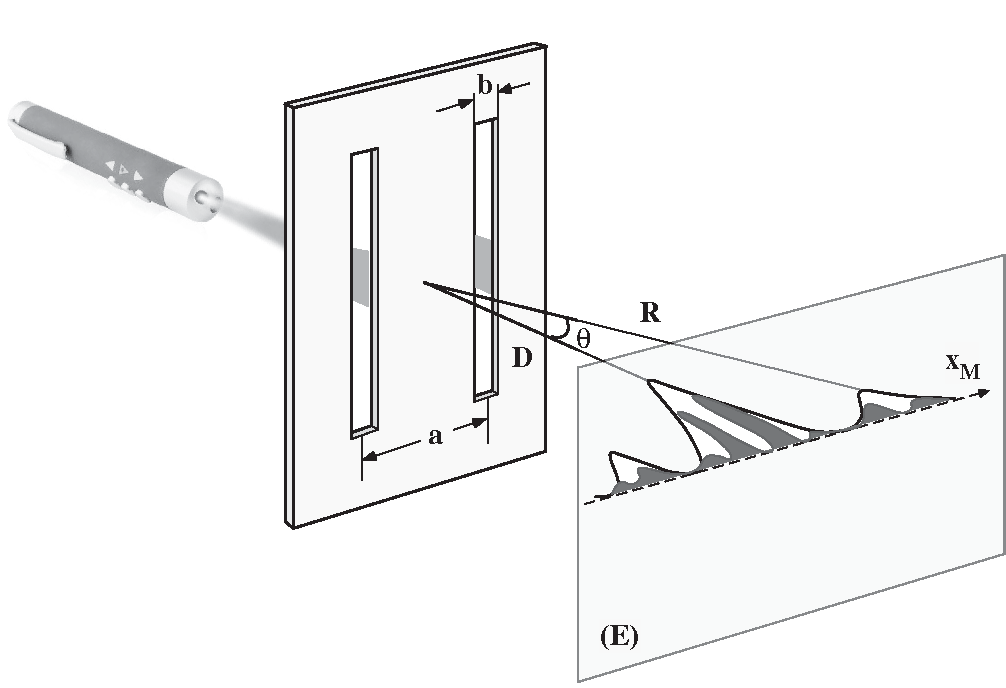
\includegraphics[width=\linewidth]{images/DoubleFente}
		\end{figure}
	\end{column}
\end{columns}
	
\begin{block}{Analytical expression}
	\begin{equation*}
	I(x) = sinc^2 (Bx)[1+cos(2Ax)] \quad \quad where: \ A = \pi a /\lambda D \ and \ B = \pi b / \lambda D
	\end{equation*}
	b stands for the width of the slits, a represents the distance between slits, D is the distance of the screen to the plan of the slits and $\lambda$ is the wavelength of the monochromatic incident light.
\end{block}


\end{frame}

\begin{frame}{Python application}
	\centering
	\animategraphics[loop,controls,width=1\linewidth]{2}{images/demo/out}{1}{118}\\
	Clone or download the code source from GitHub:\\
	\url{https://github.com/astrax/ETOP_2018}	
\end{frame}

%\begin{frame}{Python application}
%	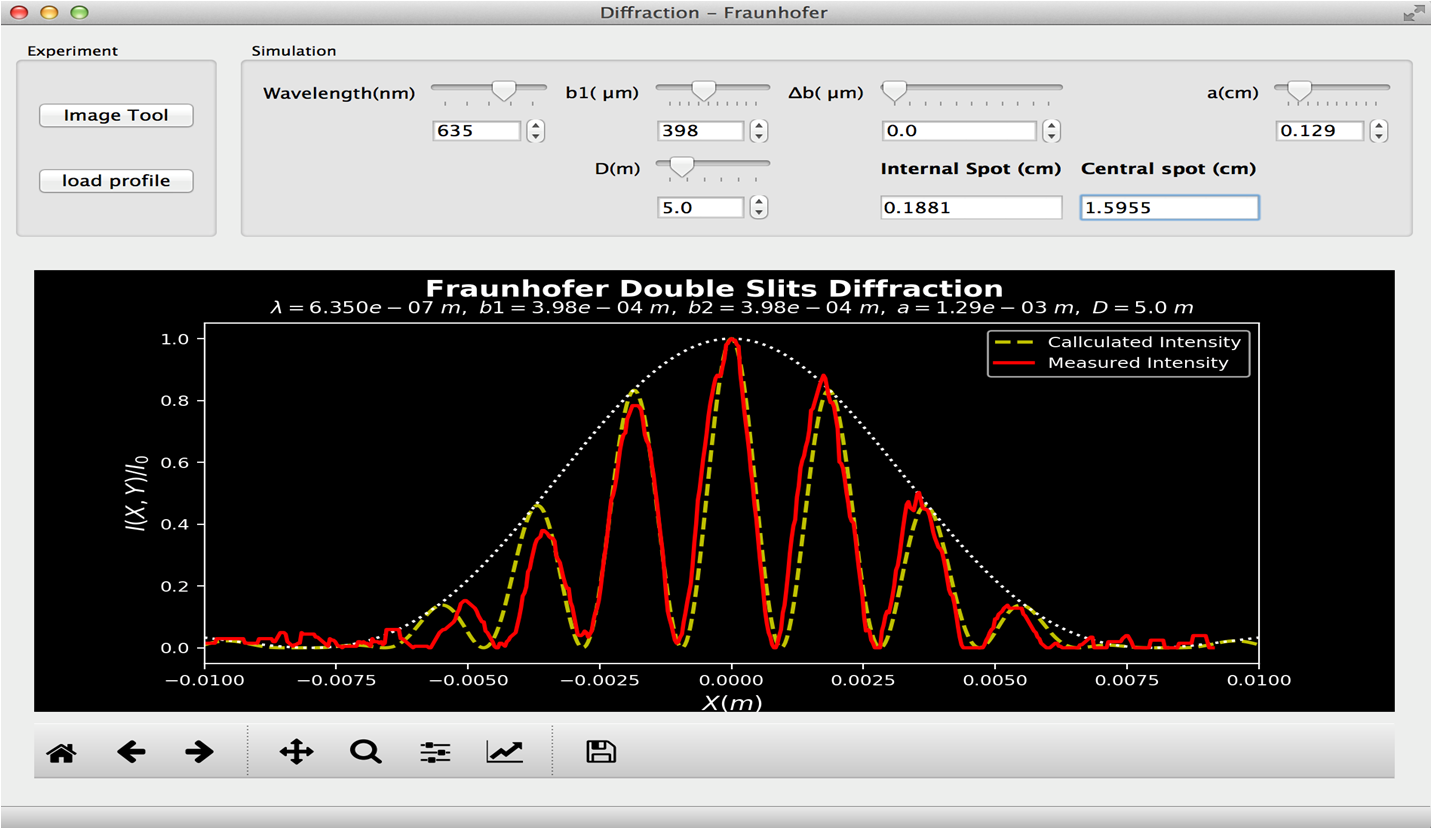
\includegraphics[width=\linewidth]{images/Image3}
%\end{frame}

\begin{frame}{New published text book}
\begin{columns}[c]
	\begin{column}{0.6\textwidth}
		More than 50 programs and applications are free to download on the book's web page: \url{www.crcpress.com/9781498755047}
		
		\begin{figure}
			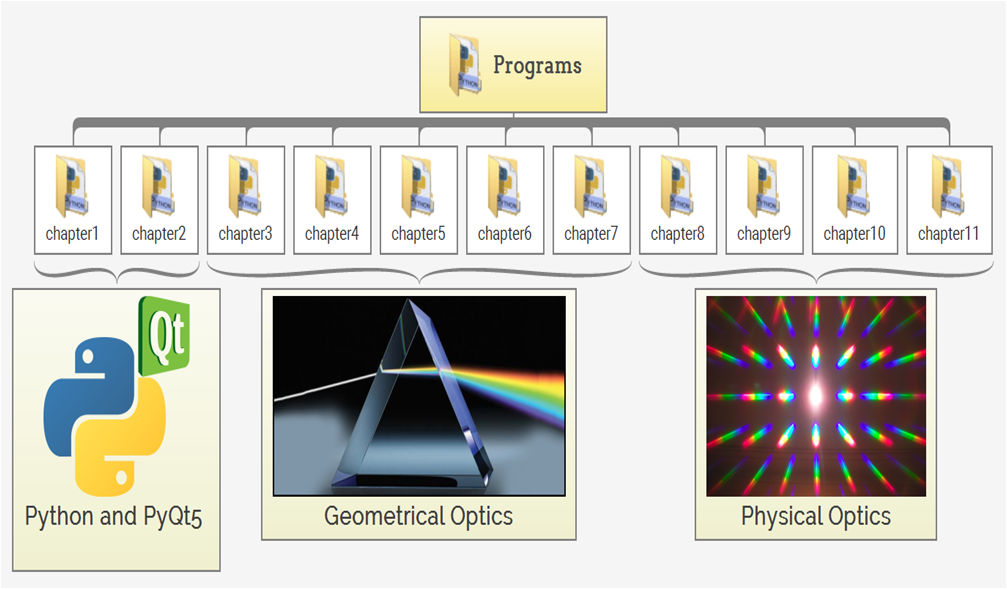
\includegraphics[width=\linewidth]{images/Image4}
			
		\end{figure}
		
		
	\end{column}
	\begin{column}{0.4\textwidth}
		\begin{figure}
			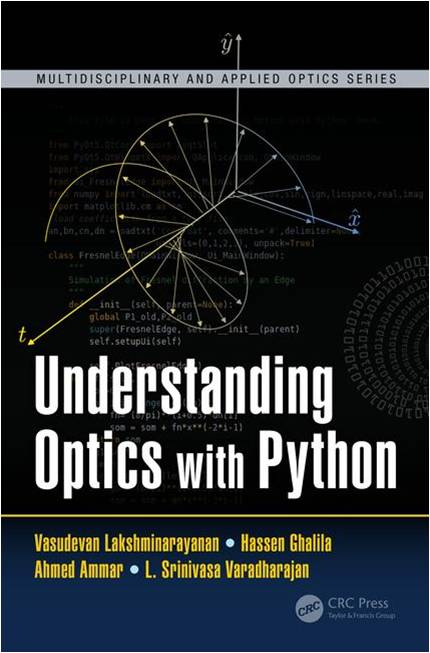
\includegraphics[width=\linewidth]{images/Image5}
			
		\end{figure}
	\end{column}
\end{columns}

\end{frame}

%\begin{frame}{Active Learning in Simulating Optics (ALSO)}
%It is essential for the student to learn the concepts behind the equations.
%\end{frame}

\begin{frame}
\centering
\huge \textbf{Thank you!}
\end{frame}

\end{document}
